\chapter{Ceros de funciones}

Los métodos numéricos nos proporcionan aproximaciones succesivas de una raíz ($\alpha$) de una función.
Comenzaremos con una aproximación inicial $x^0$  y el método nos proporcionará $x^1$. Más
generalmente, dado un $x^k$, el método nos proporcionará $x^{k+1}$.

\section{Métodos clásicos}

\subsection{Método de la bisección}

El método está basado en el teorema de Bolzano. Consiste en tomar un intervalo $(a, b)$
con $f(a)f(b) < 0$. Una vez encontrado este intervalo inicial, vamos dividiendo sucesivamente
el intervalo por la mitad y tomando el subintervalo que cumpla la condición de que sus extremos tengan
distinto signo. Reduciendo el error a la mitad.

Este método tiene la ventaja de ser muy robusto y nos permite calcular la raíz con una percisión arbitraria.
El inconveniente principal de este método es la velocidad: es un método muy lento.

\subsection{Método de Newton}

Dada una aproximación de la raíz $x^k$, calcularemos la siguiente aproximación $x^{k+1}$ como el cero de 
la recta tangente a $f$ en $x^k$, es decir, aproximaremos $f(x) \approx
f\left( x^k \right) + f^\prime\left( x^k \right) \left( x - x^k \right)$ y $x^{k+1}$ será el 0 de esta función aproximada:

\[
    x^{k+1} = x^k - \frac{f\left( x^k \right)}{f^\prime\left( x^k \right)}.
\]

La ventaja de este método es la velocidad (tiene convergencia cuadrática para raíces simples).
El inconveniente principal es que no es tan robusto: necesita una aproximación inicial suficientemente buena.
Además, este método requiere de conocer la derivada $f^\prime(x)$, lo cual puede ser costoso o imposible.

\begin{center}
    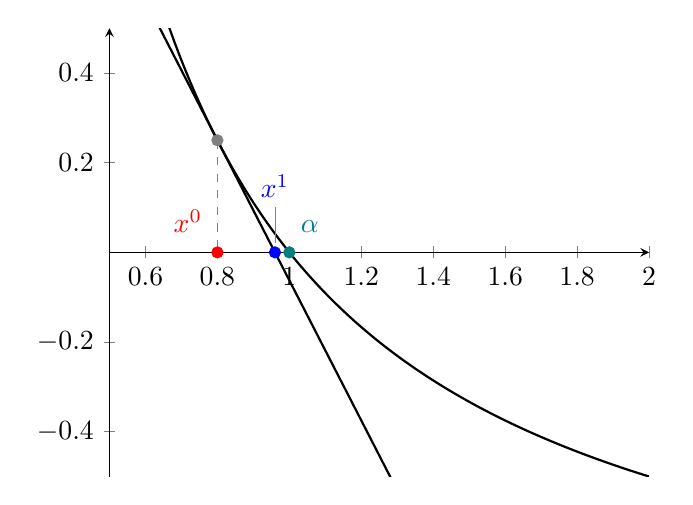
\begin{tikzpicture}
        \begin{axis}[
                xmin = 0.5,
                xmax = 2,
                ymin = -0.5,
                ymax = 0.5,
                samples = 100,
                axis lines = center
        ]
            \addplot[domain=0.5:2, thick]{1/x-1};
            \addplot[mark=*,color=gray] coordinates {(0.8, 1/0.8 - 1)} node[]{};
            \addplot[mark=*,color=red] coordinates {(0.8, 0)} node[label=120:$x^0$]{};
            \addplot[domain=0.5:2, thick]{1/0.8 - 1 + (x - 0.8)*(-1/(0.8*0.8))};
            \addplot[mark=*, color=blue] coordinates {(0.8 - (1/0.8 - 1)/(-1/(0.8*0.8)), 0)} node[pin=90:$x^1$]{};
            \addplot[mark=*, color=teal] coordinates {(1, 0)} node[label=80:$\alpha$]{};
            
	    \draw (axis cs:0.8, 1/0.8 - 1) [color=gray, dashed] -- (axis cs:0.8, 0);
        
        \end{axis}
    \end{tikzpicture}
\end{center}

\subsection{Método de la secante}

Este método parte de dos aproximaciones iniciales $x^0$ y $x^1$, tomaremos $x^2$ como el cero de la recta
que pasa por $x^0$ y $x^1$ (substituye la derivada por la recta secante). Es decir, dados $x^k$ y $x^{k-1}$,
\[
    x^{k+1} = x^k - f\left( x^k \right) \frac{x^k - x^{k-1}}{f\left( x^k \right) - f\left( x^{k-1} \right)}.
\]

Las ventajas e inconvenientes de este método son casi identicas a las del método de newton. Este método
es un poco más lento que el de Newton, aunque converge bastante rápidamente y, igual que el de Newton,
el punto flaco es que no es tan robusto como el de la bisección.

\begin{center}
    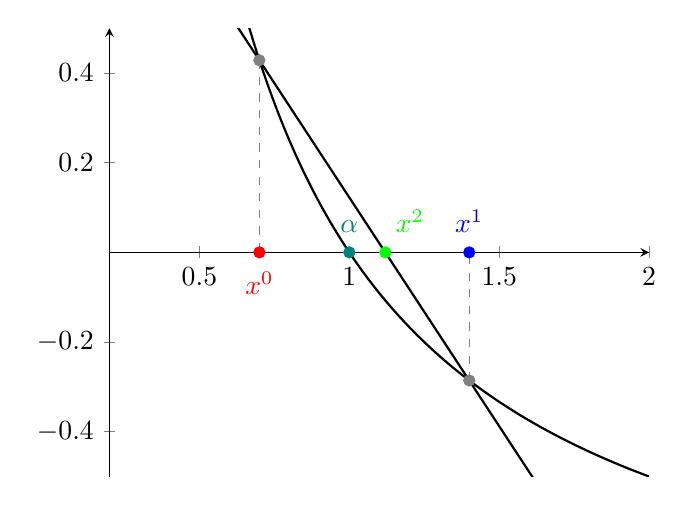
\begin{tikzpicture}
        \begin{axis}[
                xmin = 0.2,
                xmax = 2,
                ymin = -0.5,
                ymax = 0.5,
                samples = 100,
                axis lines = center
        ]
            \addplot[domain=0.5:2, thick]{1/x-1};
            \addplot[mark=*,color=gray] coordinates {(0.7, 1/0.7 - 1)} node[]{};
            \addplot[mark=*,color=gray] coordinates {(1.4, 1/1.4 - 1)} node[]{};
            
            \addplot[mark=*,color=red] coordinates {(0.7, 0)} node[label=270:$x^0$]{};
            \addplot[mark=*,color=blue] coordinates {(1.4, 0)} node[label=90:$x^1$]{};
            \addplot[domain=0.5:2, thick]{-50/49*x + 56/49};
            \addplot[mark=*, color=green] coordinates {(56/50, 0)} node[label=85:$x^2$]{};
            \addplot[mark=*, color=teal] coordinates {(1, 0)} node[label=90:$\alpha$]{};
            
            \draw (axis cs:0.7, 1/0.7 - 1) [color=gray, dashed] -- (axis cs:0.7, 0);
            \draw (axis cs:1.4, 1/1.4 - 1) [color=gray, dashed] -- (axis cs:1.4, 0);
        \end{axis}
    \end{tikzpicture}
\end{center}

\begin{obs}
    El coste computacional se mide en número de evaluaciones de $f(x)$ (y de $f^\prime(x)$).
    El método de la secante necesita 1 evaluación por iteración y por lo tanto, necesita menos que
    el método de Newton.
\end{obs}

\section{Consistencia y convergencia}

\begin{defi}[método!consistente]
    Diremos que un método $x^{k+1} = \phi\left( x^k \right)$ es consistente si las raíces son
    los únicos puntos fijos, es decir,
    \[
        f(\alpha) = 0 \iff \phi(\alpha) = \alpha.
    \]
\end{defi}

\begin{ej}
    Un ejemplo es el método de Newton.

    Si $\alpha$ es una raíz simple,
    \[
        f(\alpha) = 0 \implies \phi(\alpha) = \alpha - \frac{f(\alpha)}{f^\prime(\alpha)} = \alpha.
    \]
    Por otro lado,
    \[
        \phi(\alpha) = \alpha \implies \frac{f(\alpha)}{f^\prime(\alpha)} = 0 \implies f(\alpha) = 0.
    \]
    Con la raíz doble, no podemos evaluar el método de Newton en $\alpha$, pero por la regla de l'Hôpital llegaríamos
    a la conclusión de que, tomando el límite de $\phi$ se sigue cumpliendo.

    Análogamente, podemos deducir que el método de Newton es un método consistente para una raíz $\alpha$ de
    cualquier múltiplicidad.
\end{ej}

\begin{defi}[método!convergente]
    Diremos que un esquema es convergente si
    \[
        \lim_{k \to \infty} x^k = \alpha.
    \]
\end{defi}

\begin{defi}[error!absoluto]
    Llamaremos error absoluto de la aproximación a 
    \[
        E^k = \abs{x^k - \alpha}
    \]
    y es equivalente que el método sea convergente a que $\lim\limits_{k \to \infty} E^k = 0$.
\end{defi}

\begin{defi}[convergencia!lineal]
    Diremos que un esquema tiene convergencia lineal si
    \[
        \abs{E^{k+a}} \leq \lambda \abs{E^k}, \; \lambda < 1.
    \]
\end{defi}

\begin{defi}[convergencia!de orden $p$]
    Diremos que un esquema tiene convergencia de orden $p$ si
    \[
        \abs{E^{k+1}} \leq \lambda \abs{E^k}^p.
    \]
\end{defi}

\begin{defi}[convergencia!superlineal]
    Diremos que un esquema tiene convergencia superlineal si
    \begin{gather*}
        \abs{E^{k+a}} \leq \lambda_k \abs{E^k}, \; \lambda_k \to 0 \\
        \text{o bien} \\
        \abs{E^{k+1}} \leq \lambda \abs{E^k}^q, \; q \in (1, 2).
    \end{gather*}
\end{defi}

\begin{prop}
    Para estudiar la convergencia, en general, necesitamos estudiar $E^{k+1}$ en función de $E^k$.
    Para ello, podemos usar la siguiente fórmula:
    \[
        E^{k+1} = \phi^\prime(\alpha)E^k + \frac{1}{2} \phi^{\prime \prime}(\alpha)\left( E^k \right)^2 - \cdots
    \]
    o más generalmente
    \[
        E^{k+1} = \sum^{\infty}_{i = 1} \frac{1}{i!} \phi^{(i)}(\alpha) \left( E^k \right)^i.
    \]
\end{prop}

\begin{proof}
    Tenemos que
    \[
        E^{k+1} = x^{k+1} - \alpha = \phi(x^k) - \phi(\alpha)
    \]
    Aproximando ahora por Taylor (centrado en $\alpha$):
    \[
        E^{k+1} = \cancel{-\phi(\alpha)} + \cancel{\phi(\alpha)} + \phi^\prime(\alpha)(x^k - \alpha) + \dots
    \]
    substituyendo ahora $x^k - \alpha = E^k$, obtenemos la fórmula original.
\end{proof}

\begin{prop}
    Si $\phi^\prime(\alpha) \neq 0$ y $\abs{\phi(\alpha)} < 1$, entonces el método converge linealmente.
\end{prop}

\begin{proof}
    Veremos ahora que la convergencia es lineal:
    \[
        \abs{E^{k+1}} \leq \abs{E^k} \left( \abs{\phi^\prime(\alpha)} + 
            \underbrace{\abs{\frac{1}{2} \phi^{\prime \prime}(\alpha)} E^k +
            \O\left( \left( E^k \right)^2 \right)}_{\leq \varepsilon} \right).
    \]
    Consideramos $\varepsilon$ tal que $\abs{\phi^\prime(\alpha)} + \varepsilon \leq 1$. Esto pasa
    si $\abs{E^k}$ es suficientemente pequeño. Entonces
    \[
        \abs{E^{k+1}} \leq \lambda \abs{E^k},
    \]
    con $\lambda = \abs{\phi^\prime} + \varepsilon < 1$.
\end{proof}

\begin{prop}
    Si $\phi^\prime(\alpha) = \cdots = \phi^{(p-1)}(\alpha) = 0$ y $\phi^{(p)}(\alpha) = 0$. Tenemos que
    \[
        E^{k+1} = \frac{1}{p!}\phi^{(p)}(\alpha) \left( E^k \right)^p +
        \frac{1}{(p+1)!} \phi^{(p+1)}(\alpha) \left( E^k \right)^{p+1} + \dots
    \]
    Entonces, para $E^k$ pequeño, se tiene que
    \[
        \abs{E^{k+1}} \approx \abs{\frac{\phi^{(p)}(\alpha)}{p!}} \left( E^k \right)^p
    \]
    y la convergencia es de orden $p$.
\end{prop}

\begin{proof}
    Se tiene que
    \[
        \abs{E^{k+1}} \leq \abs{E^k} \left( \abs{\frac{\phi^{(p)}(\alpha)}{p!}} +
        \underbrace{\abs{\frac{\phi^{(p+1)}(\alpha)}{(p+1)!}} \left( E^k \right) +
        \O\left( \left( E^k \right)^2 \right)}_{\leq \varepsilon} \right).
    \]
    Con $\abs{E^k}$ suficientemente pequeño
    \[
        \abs{E^{k+1}} \leq \left( \abs{E^k} \right)^p
        \underbrace{\left( \frac{\phi^{(p)}(\alpha)}{p!} + \varepsilon  \right)}_{\lambda}.
    \]
\end{proof}

\begin{defi}[factor asintótico de convergencia]
    Sea $\phi$ un método lineal, por lo tanto,
    \[
        \abs{E^{k+1}} \leq \lambda \abs{E^k}.
    \]
    Llamaremos factor asintótico de convergencia a $\lambda$.
\end{defi}

\subsection{Análisis del método de Newton}

Para estudiar la convergencia, primero es conveniente, conocer las derivadas de la función $\phi$, así pues,
tenemos
\[
    \begin{aligned}
        \phi(x) &= x - \frac{f(x)}{f^\prime(x)}, \\
        \phi^\prime(x) &= \frac{f(x)f^{\prime \prime}(x)}{f^\prime(x)^2}, \\
        \phi^{\prime \prime}(x) &= \frac{f^{\prime \prime}(x)}{f^\prime(x)} -
        \frac{2 f(x)f^{\prime \prime}(x)^2}{f^\prime(x)^3} +
        \frac{f(x)f^{\prime \prime \prime}(x)}{f^\prime(x)^2}.
    \end{aligned}
\]
\begin{itemize}
    \item Caso de una raíz simple, $f(\alpha) = 0$ y $f^\prime(\alpha) \neq 0$.
        En este caso,
        \[
            \begin{aligned}
                \phi^\prime(\alpha) &= 0, \\
                \phi^{\prime \prime}(\alpha) &= \frac{f^{\prime \prime}(\alpha)}{f^\prime(\alpha)}.
            \end{aligned}
        \]
        En general $\phi^{\prime \prime}(\alpha) \neq 0$, por lo tanto el método de Newton
        tiene, en general, convergencia de orden 2.
    \item Caso de una raíz doble $f(\alpha) = f^\prime(\alpha) = 0$ y $f^{\prime \prime}(\alpha) \neq 0$.
        Observamos que $\phi^\prime(\alpha)$ no está bien definido, pero podemos calcular el límite, teniendo
        \[
            \begin{aligned}
                \lim_{x \to \alpha} \phi^\prime(x) &= \lim_{x \to \alpha} \frac{f(x)f^{\prime \prime}(x)}{f^\prime(x)^2}
                \stackrel{\text{R.H.}}{=} \lim_{x \to \alpha}
                \frac{f^\prime(x)f^{\prime \prime}(x) + f(x)f^{\prime \prime \prime}(x)}
                {2 f^\prime(x)f^{\prime \prime}(x)} = \\ &= \lim_{x \to \alpha} 
                \frac{f^\prime(x)f^{\prime \prime}(x)}{2 f^\prime(x) f^{\prime \prime}(x)} +
                \frac{f(x)f^{\prime \prime \prime}(x)}{2 f^\prime(x)f^{\prime \prime}(x)} =
                \frac{1}{2} + \lim_{x \to \alpha} \frac{f(x)f^{\prime \prime \prime}(x)}
                {2f^\prime(x)f^{\prime \prime}(x)} \stackrel{\text{R.H.}}{=} \\ &= \frac{1}{2} +
                \lim_{x \to \alpha} \frac{f^\prime(x)f^{\prime \prime \prime}(x) + f(x)f^{(4)}(x)}
                {2f^{\prime \prime}(x)^2 + 2f^\prime(x)f^{\prime \prime \prime}(x)} = \frac{1}{2}.
            \end{aligned}
        \]
        Por lo tanto es lineal con factor asintótico de convergencia igual a $\frac{1}{2}$.

    \item El caso de multiplicidad $p$, es decir, $f(\alpha) = \cdots = f^{(p-1)}(\alpha) = 0$ y
        $f^{(p)} \neq 0$. Para resolver este caso, aplicaremos $p-2$ veces la regla de L'Hôpital
        \[
            \begin{aligned}
                \lim_{x \to \alpha} \phi^\prime(x) &= \lim_{x \to \alpha} \frac{f(x)f^{\prime \prime}(x)}{f^\prime(x) f^\prime(x)}
                \stackrel{\text{Leibniz}}{=} \lim_{x \to \alpha} \frac{\sum\limits^{p-2}_{k = 0} {p-2 \choose k}
                f^{(2p-k)}(x)f^{(k)}}{\sum\limits^{p-2}_{k = 0} {p-2 \choose k }f^{(2p-1-k)}(x)f^{(k+1)}(x)} = \\
                &= \lim_{x \to \alpha} \frac{{2p-2 \choose p} \cancel{f^{(p)}(x)f^{(p)}(x)}}
                {{2p-2 \choose p-1}\cancel{f^{(p)}(x)f^{(p)}(x)}} =
                \frac{ {2p-2 \choose p} }{ {2p-2 \choose p-1} } = \frac{(p-1)!(p-1)!}{p!(p-2)!} = \\
                &= \frac{p-1}{p} = 1 - \frac{1}{p}.
            \end{aligned}
        \]
        El método es lineal con F.A.C. igual a $1 - \frac{1}{p}$.
\end{itemize}

\subsection{Gráficos de convergencia}

\begin{defi}[error!relativo]
    Definimos el error relativo como
    \[
        r^k = \frac{E^k}{\alpha} = \frac{x^k - \alpha}{\alpha}.
    \]
\end{defi}
\begin{obs}
    $x^k$ tiene $q$ cifras significativas correctas si $\abs{r^k} \leq \frac{1}{2} 10^{-q}$.
\end{obs}
\noindent Caso de convergencia lineal
\begin{align*}
    \abs{E^{k+1}} &\approx \lambda \abs{E^k},\, \lambda = F.A.C. \stackrel{x^{k+1} = \phi(x^k)}{=} \abs{\phi'(\alpha)}, \\
    \frac{\abs{E^k}}{\abs{\alpha}} &\approx \lambda^k\frac{\abs{E^0}}{\abs{\alpha}} \implies \abs{r^k} \approx \lambda^k\abs{r^0}.
\end{align*}

\noindent Si la convergencia es de orden $p \geq 2$,
\begin{align*}
	\abs{E^k} &\approx \lambda \left( \abs{E^{k-1}} \right)^p \approx \lambda \left( \lambda \abs{E^{k-2}}^p \right)^p = \lambda^{1+p} \abs{E^{k-2}}^{p^2} \approx \lambda^{p+1} \left( \lambda\abs{E^{k-3}}^p \right)^{p^2} = \dots \\
    &\approx \lambda^{1+p+\dots+p^{k-1}} \abs{E^0}^{p^k} \stackrel{\text{serie geométrica}}{=} \lambda^{\frac{p^k-1}{p-1}} \abs{E^0}^{p^k}, \\
    \frac{\abs{E^k}}{\abs{\alpha}} &\approx \lambda^{\frac{p^k-1}{p-1}}\frac{\abs{E^0}^{p^k}}{\abs{\alpha}^{p^k}}\abs{\alpha}^{p^k-1}, \\
    \abs{r^k} &\approx A^{p^k}\cdot B, \\
    \log \abs{r^k} &\approx \log B + p^k\log A, \,\text{donde }A = \lambda^{\frac{1}{p-1}}\abs{r^0}\abs{\alpha}, \, B = \lambda^{\frac{-1}{p-1}} \abs{\alpha}^{-1}.
\end{align*}
\begin{example}
    El error nos proporciona información sobre el tipo de convergencia.
    \begin{center}
        \begin{tabular}{|c|c|c|} \hline
            & \begin{tabular}{@{}c@{}}Bisección \\ (lineal $\lambda = \sfrac{1}{2}$) \end{tabular} & \begin{tabular}{@{}c@{}}Newton \\ (cuadrática) \end{tabular} \\ \hline\hline
            $|r^0|$ & $0,1 \cdot 10^{-1}$ & $0,1\cdot 10^{-1}$ \\\hline
            $|r^1|$ & $0,5 \cdot 10^{-2}$ & $0,1\cdot 10^{-2}$ \\\hline
            $|r^2|$ & $0,25 \cdot 10^{-2}$ & $0,1\cdot 10^{-4}$ \\\hline
            $|r^3|$ & $0,12 \cdot 10^{-2}$ & $0,1\cdot 10^{-8}$ \\\hline
        \end{tabular}
    \end{center}
\end{example}

\subsection{Criterios prácticos de convergencia}
\noindent Si queremos $q$ cifras significativas correctas (C.S.C.), pararemos el algoritmo cuando
\[
    \frac{1}{2}10^{-q} > \abs{r^k} = \frac{\abs{x^k - \alpha}}{\abs{\alpha}} \stackrel{\alpha\approx x^{k+1}}{\approx} \frac{\abs{x^k-x^{k+1}}}{\abs{x^{k+1}}}.
\]
En caso que $\alpha \approx 0$, podemos hacer una variación
\[
    \abs{x^k-\alpha} < \varepsilon\abs{x^k} + \varepsilon.
\]
Conviene comprobar el error en el ``residuo'' $f\left( x \right)$. El criterio puede ser combinado
\[
    \abs{x^k-\alpha} + \abs{f\left( x^k \right)} < \varepsilon_f.
\]

\section{Métodos híbridos}

\noindent Método de Brent: véase \href{https://en.wikipedia.org/wiki/Brent\%27s_method}{Brent's method - Wikipedia}.
